\section{Worked examples: $N=16$}
\label{sec:examples}

All examples in this section are built from 16 real 32-byte pseudorandom
elements, hashed with a toy but real compression function ($C(s,b) =
\mathrm{SHA256}(0x01 \,\Vert\, s \,\Vert\, b)$, 32-byte state and block --
so $b=w$, using the identity checkpoint encoding $\mathrm{pad}_w(x)=x$ of
Definition~\ref{def:padb} rather than the $b>w$ terminator-byte scheme),
and every proof below was independently re-verified, including confirming
that flipping a single bit anywhere in the target data, or in any one
revealed value, is rejected.

\begin{table}[htbp]
\centering
\begin{tabular}{@{}cccc@{}}
\toprule
Target index & Base pair proved (both) & Reveals & Proof size \\
\midrule
0  & $D[0],D[1]$   & 3 & 160 B \\
4  & $D[4],D[5]$   & 3 & 160 B \\
7  & $D[6],D[7]$   & 3 & 160 B \\
8  & $D[8],D[9]$   & 3 & 160 B \\
11 & $D[10],D[11]$ & 3 & 160 B \\
14 & $D[14],D[15]$ & 3 & 160 B \\
\bottomrule
\end{tabular}
\caption{Six representative target indices out of the 16 possible, spread
across the file; all 16 were checked and every one produces the same
\emph{constant} 160-byte proof ($2 \times 32$ bytes of raw pair data plus
$3 \times 32$ bytes of state reveals, $L-1=3$), since proof size does not
depend on which index is targeted (Section~\ref{sec:algorithm}). A proof
for target index $a$ always discloses \emph{both} raw elements of its base
pair, $D[a_0]$ and $D[a_0{+}1]$ -- proving index 7 necessarily also
discloses element 6 -- so the ``Base pair proved'' column names both
elements the proof exposes, not just the requested index (Section~\ref{sec:algorithm-cost}
discusses this). For comparison, a same-shape Merkle proof over 16 leaves
needs $\lceil \log_2 16 \rceil = 4$ sibling hashes (128 bytes) plus the
leaf's own preimage, and does \emph{not} disclose a neighboring leaf.}
\label{tab:examples-n16}
\end{table}

\subsection{Index 7 in detail}

Figure~\ref{fig:proof-n16-idx7} shows the full 16-element structured file
with the proof path for index 7 highlighted: the base pair $D[6],D[7]$,
and the checkpoint values $\CK_4$, $\CK_6$, and $\CK_{[12,15]}$, in the
order the proof actually reveals them.

\begin{figure}[htbp]
\centering
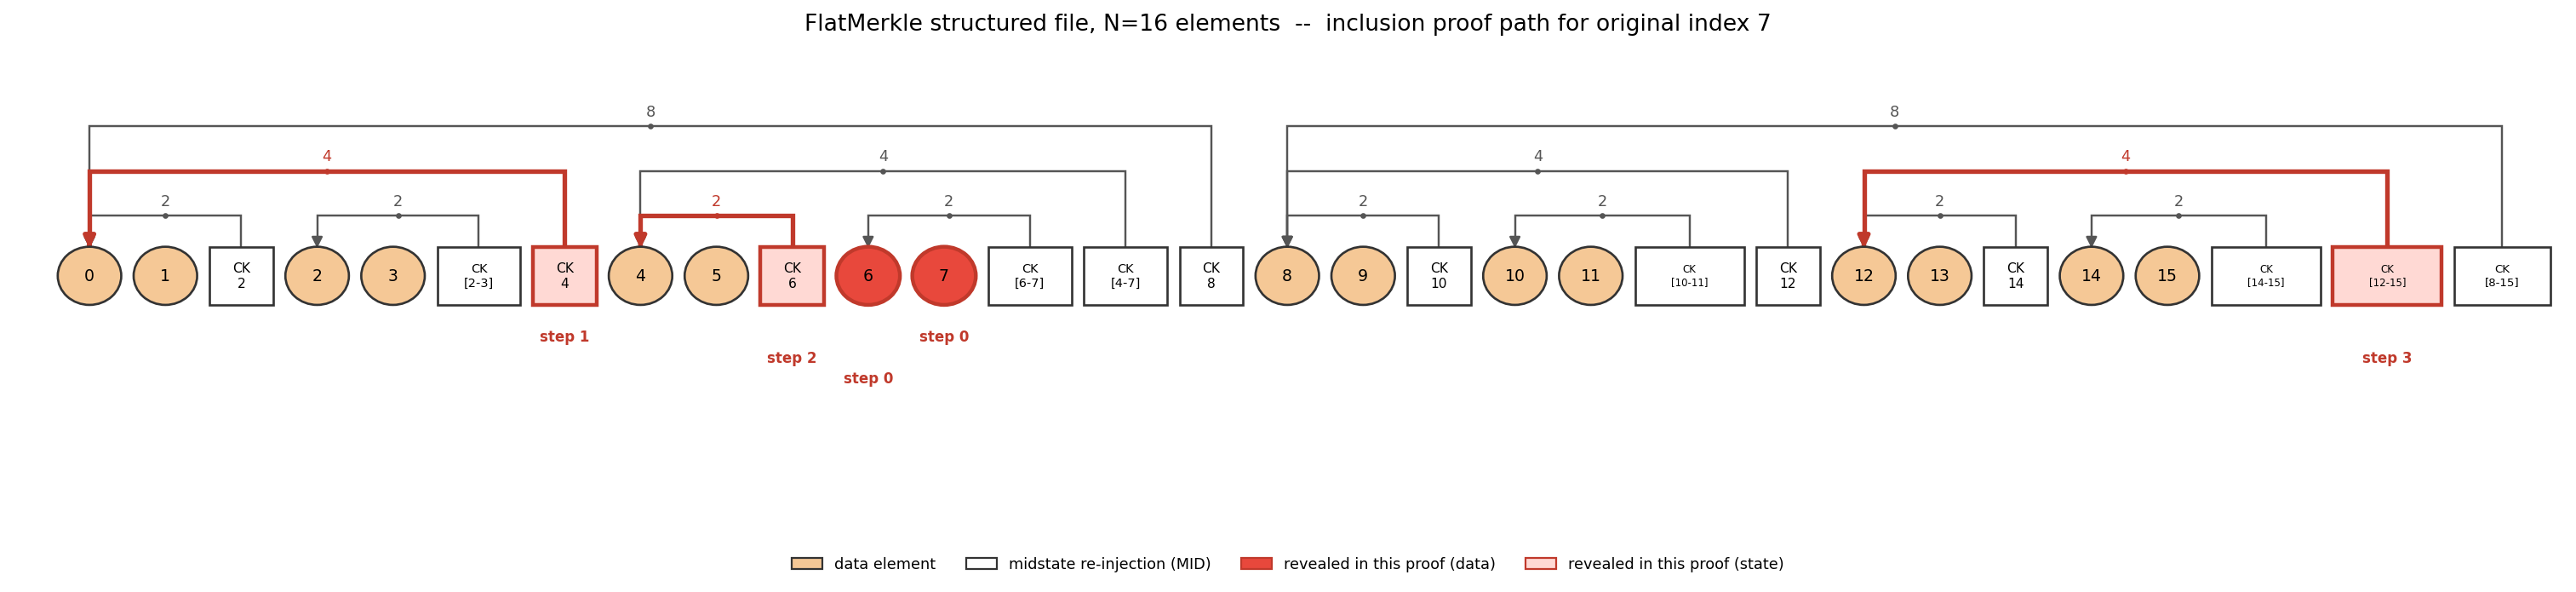
\includegraphics[width=\textwidth]{figures/proof_n16_idx7.png}
\caption{Structured file for $N=16$, proof path for index 7 highlighted in
red, numbered by the order each value is used.}
\label{fig:proof-n16-idx7}
\end{figure}

A natural question when first looking at Figure~\ref{fig:proof-n16-idx7} is
how the verifier gets from ``just after element 7'' to the digest: no arc
in the drawing runs directly from that point to the end. The reason is that
the verifier does not walk the file's own drawn jump-back arcs at all -- it
performs a straight, ordered fold of $\C(\cdot,\cdot)$ calls, each combining
the previous result with either the next raw element or the next revealed
checkpoint. Figure~\ref{fig:chain-n16-idx7} makes this explicit.

\begin{figure}[htbp]
\centering
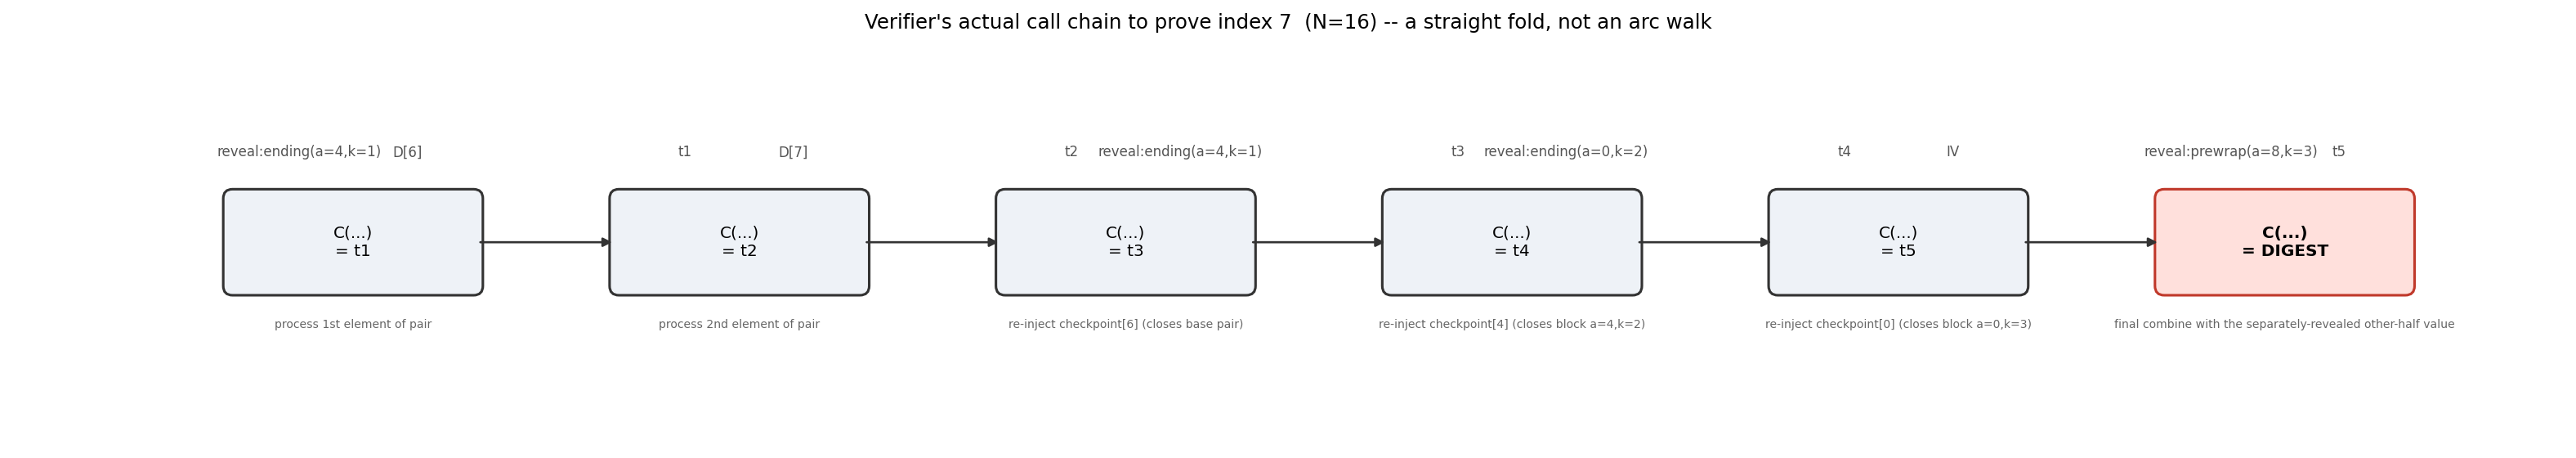
\includegraphics[width=\textwidth]{figures/chain_n16_idx7.png}
\caption{The verifier's actual sequence of compression-function calls for
index 7 -- a straight-line fold ending at the digest, not a walk along the
structured file's own arcs.}
\label{fig:chain-n16-idx7}
\end{figure}

Finally, Figure~\ref{fig:proof-stored-n16-idx7} shows the proof exactly as
it is stored and transmitted: a flat, ordered sequence of items with no tree
and no arcs, matching the compact wire format
\[
(D[a_0],\ D[a_0{+}1],\ \mathrm{reveals}[0..L{-}2]),
\]
where $a_0 = a - (a \bmod 2)$ is derived by the verifier from whichever
index it is asking about, never transmitted as part of the proof itself
(Remark~\ref{rem:a0-bug} explains why the proof must not carry its own
copy of $a_0$).

\begin{figure}[htbp]
\centering
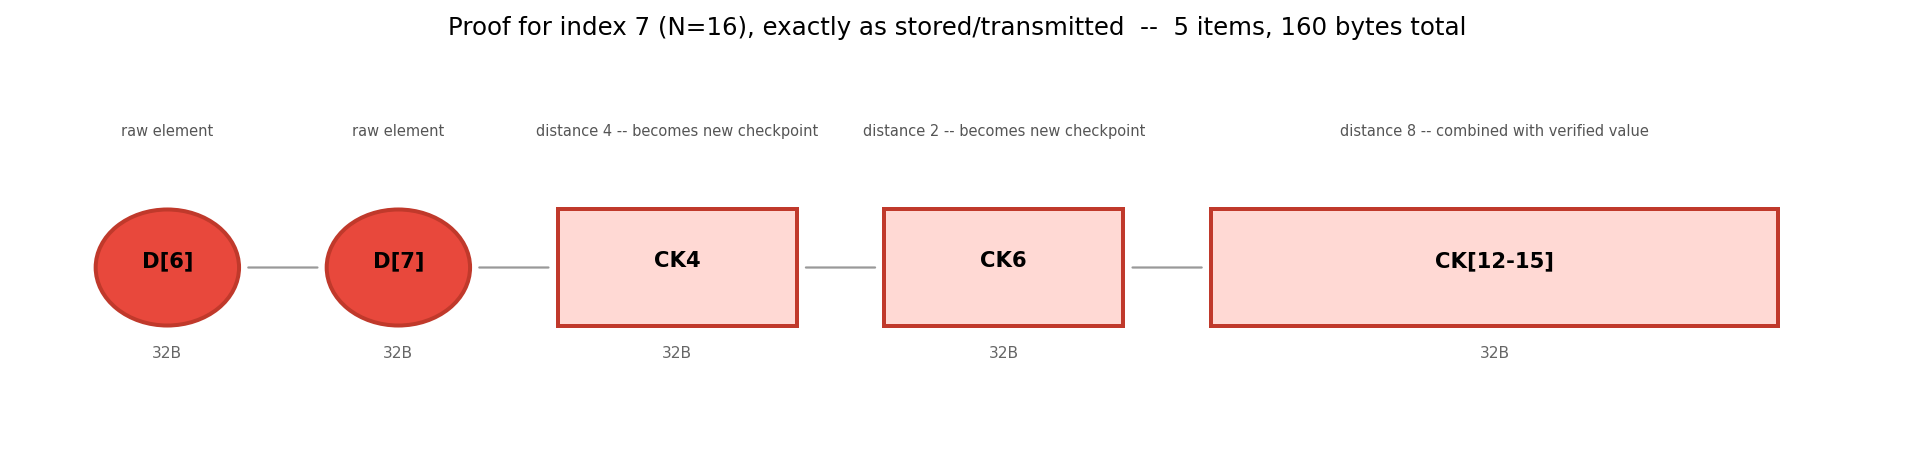
\includegraphics[width=0.8\textwidth]{figures/proof_stored_n16_idx7.png}
\caption{The index-7 proof exactly as stored: $D[6], D[7], \CK_4, \CK_6, \CK_{[12,15]}$ -- 5 items, 160 bytes, verified byte-for-byte against the real prover output.}
\label{fig:proof-stored-n16-idx7}
\end{figure}

\subsection{Reading the checkpoint labels}

$\CK_4$ and $\CK_6$ are each a single, unambiguous position: each is the
closing value ($\mathrm{ending}$) of a \emph{left}-child block, immediately
promoted to the checkpoint that starts the next block
(Section~\ref{sec:construction}). Using a single trailing index for this
kind of value (e.g.\ naming it by the last element it covers) would be
ambiguous, since different-sized blocks can share the same last-covered
index; the span notation avoids that collision by construction.

$\CK_{[12,15]}$ is different in kind, and worth reading carefully. The
third reveal is $\mathrm{prewrap}(8,3)$ -- the state right before
$\mathrm{block}(8,3)$'s own closing $\mathrm{MID}(8)$ folds in, \emph{not}
$\mathrm{ending}(8,3)$ (which is the file's own final raw chain state, and
is never revealed to any verifier, since it only exists after the
verifier's own last fold). $\mathrm{prewrap}(8,3)$ happens to equal
$\mathrm{ending}(12,2)$ -- $\mathrm{block}(8,3)$'s own right child's ending,
one level down -- since that child closes immediately before
$\mathrm{block}(8,3)$'s own $\mathrm{MID}(8)$ is written, so it names the
right child's span, $\CK_{[12,15]}$, \emph{not} $\mathrm{block}(8,3)$'s own
span $\CK_{[8,15]}$ (which would name a value -- $\mathrm{ending}(8,3)$ --
this proof never touches at all). The verifier does not receive
$\CK_{[12,15]}$ as a promoted checkpoint the way it does $\CK_4$ or
$\CK_6$: it folds this reveal together with $D[6],D[7]$'s already-verified
result to \emph{compute} $\mathrm{block}(8,3)$'s own closing value, which
the verifier itself performs as the last fold in
Figure~\ref{fig:chain-n16-idx7}.
